\documentclass[11pt,fleqn]{exam}
\usepackage[utf8]{inputenc}

\usepackage[margin=1in]{geometry}
\usepackage{amsmath,amssymb}
\usepackage{gensymb}
\usepackage{multicol}
\usepackage{float}
\usepackage{graphicx}
\usepackage{units,icomma}
\usepackage[colorlinks,linkcolor=blue,urlcolor=blue]{hyperref}
\usepackage[margin=1.5cm]{caption}


%\usepackage{lipsum}
\usepackage[printwatermark]{xwatermark}
\usepackage{xcolor}
\usepackage{graphicx}
\newwatermark[allpages,color=blue!10,angle=45,scale=2,xpos=0,ypos=0]{ridlow.wordpress.com}

\hyphenation{
  chro-no-ampe-ro-met-ric
  ber-dia-me-ter
  de-ngan
  me-nem-pati
  mic-ro-graphs
  di-ban-ding}

\renewcommand{\figurename}{Gambar.}
\def\equationautorefname{Persamaan}
\newcommand{\class}{OLIMPIADE ASTRONOMI}
\newcommand{\term}{Tingkat Kabupaten/Kota - 2018}
\newcommand{\examnum}{OSK Astronomi 2018}
%\newcommand{\examdate}{11/02/2014}
%\newcommand{\timelimit}{120 Minutes}

\pagestyle{head}
\firstpageheader{}{}{}
\runningheader{\examnum}{}{Halaman \thepage\ dari \numpages}
\runningheadrule


\begin{document}

\noindent
\begin{tabular*}{\textwidth}{l @{\extracolsep{\fill}} r @{\extracolsep{6pt}} l}
\textbf{\class} \\% & \textbf{Name:} & \makebox[2in]{\hrulefill}\\
\textbf{\term}  %&&\\
%\textbf{\examnum} &&\\
%\textbf{\examdate} &&\\
%\textbf{Time Limit: \timelimit} & Teaching Assistant & \makebox[2in]{\hrulefill}
\end{tabular*}\\
\rule[2ex]{\textwidth}{2pt}

\noindent
\begin{tabular}{ll}
Copyright (c) 2018 & Ridlo W. Wibowo (ridlo.w.wibowo@gmail.com)\\
                   & Sulistiyowati (sulis.astro08@gmail.com)
\end{tabular}

\vspace{0.3cm}
\noindent
Solusi ini dibuat tanpa jaminan kesesuaian dengan solusi resmi dari juri olimpiade sains bidang Astronomi. Pengguna boleh menyebarluaskan dan/atau memodifikasi solusi ini dengan mencantumkan sumber asli. Hak cipta soal ada pada Kemendiknas dan dilindungi undang-undang.

\vspace{0.4cm}
\noindent
\rule[2ex]{\textwidth}{1.5pt}

\textbf{Soal Pilihan Ganda}

\begin{questions}
\question Nilai dari 
$$\lim_{n \rightarrow \infty} \frac{\sin^3{n}}{n}$$
adalah
\begin{choices}
\choice -1
\choice 0
\choice 1
\choice $\infty$
\choice Tidak ada solusi
\end{choices}

\textit{Jawaban: } B

Berapapun nilai $n$, nilai $\sin(n)$ dan juga $\sin^3(n)$ akan tetap berada di rentang -1 dan 1. Pada persamaan tersebut nilai pembagi $n$ akan terus bergerak menuju tak hingga. Sehingga nilai limitnya adalah 0.  


\question Terdapat 28 bintang dalam suatu daerah berbentuk segitiga yang dibatasi oleh tiga titik: $A$(2 pc, 0, 0), $B$(0, 4 pc, 0), dan $C$(0, 0, 6 pc). Jumlah bintang per pc$^2$ daerah tersebut adalah 
\begin{choices}
\choice 1
\choice 2
\choice $\frac{28}{35} \sqrt{7}$
\choice $\frac{28}{\sqrt{235}}$
\choice Tidak ada yang benar
\end{choices}

\textit{Jawaban: } B

\textbf{Cara 1}:

Untuk mengetahui rapat jumlah bintang, tentu kita perlu menghitung luas segitiga $\triangle ABC$ terlebih dahulu. Jika kita gambar titik-titiknya dalam koordinat kartesian (3D), maka akan dengan mudah dapat kita cari panjang sisi segitiga ini,
\begin{itemize}
\item panjang AB = $\sqrt{(2-0)^2 + (0-4)^2 + (0-0)^2} = \sqrt{20}$

\item panjang AC = $\sqrt{(2-0)^2 + (0-0)^2 + (0-6)^2} = \sqrt{40}$

\item panjang BC = $\sqrt{(0-0)^2 + (4-0)^2 + (0-6)^2} = \sqrt{52}$
\end{itemize}

Luas segitiga dapat dicari dengan rumus Heron,
\begin{eqnarray*}
\text{Luas } \triangle ABC = \sqrt{s(s-a)(s-b)(s-c)}
\end{eqnarray*}
dengan $s = \frac{a + b + c}{2}$, dan $a$, $b$, $c$, adalah panjang sisi-sisi segitiga. Langsung pakai saja kalkulator! Hasilnya luas $\triangle ABC$ adalah 14. Rapat jumlah bintangnya menjadi 28/14 = 2 bintang/pc$^2$.

\textbf{Cara 2}:

Kita bisa cari vektor yang membangun segitiga ini, misal vektor $\overrightarrow{AB}$, dan vektor $\overrightarrow{AC}$, luas segitiga bisa dicari dengan menghitung hasil perkalian \textit{cross} dua vektor ini dibagi dua. Hal ini dapat dilakukan karena hasil perkalian $cross$ dua vektor merupakan vektor yang ``panjang''nya adalah luas jajar genjang yang terbentuk oleh dua vektor tersebut
$$\left\vert \overrightarrow{AB} \times \overrightarrow{AC} \right\vert = \left\vert \overrightarrow{AB} \right\vert \left\vert \overrightarrow{AC} \right\vert \sin{\theta} \quad \rightarrow \quad \text{(luas jajar genjang)}$$

Sehingga, luas segitiga dapat dicari dengan 
$$\frac{1}{2} \left\vert \overrightarrow{AB} \times \overrightarrow{AC} \right\vert$$

Vektor $\overrightarrow{AB} = (0, 4, 0) - (2, 0, 0) = (-2, 4, 0)$

Vektor $\overrightarrow{AC} = (0, 0, 6) - (2, 0, 0) = (-2, 0, 6)$

\begin{eqnarray*}
\overrightarrow{AB} \times \overrightarrow{AC} &=& \left\vert 
\begin{array}{ccc}
i & j & k \\
-2 & 4 & 0 \\
-2 & 0 & 6
\end{array}
\right\vert = (24 - 0)i + (0 - -12)j + (0 - -8)k\\
&=& 24i + 12j + 8k
\end{eqnarray*}
\begin{eqnarray*}
\text{Luas } \triangle ABC &=& \frac{1}{2} \left\vert \overrightarrow{AB} \times \overrightarrow{AC} \right\vert \\
&=& \frac{1}{2} \cdot \sqrt{24^2 + 12^2 + 8^2}\\
&=& \frac{1}{2} \cdot \sqrt{784}\\
&=& \frac{1}{2} \cdot 28 \\
&=& 14
\end{eqnarray*}
Rapat jumlah bintangnya menjadi 28/14 = 2 bintang/pc$^2$.



\question Pengamat spektroskopik \textit{Supernova Remnant} pada rentang panjang gelombang sinar-X menunjukkan garis-garis emisi bukti peluruhan atom Titanium-44 ($^{44}$Ti). Diketahui massa awal atom $^{44}$Ti tersebut $3,1 \times 10^{-4} M_{\odot}$, waktu paruh atom tersebut adalah 60 tahun, dan umur \textit{Supernova Remnant} sekitar 5000 tahun. Tentukan berapa kelimpahan atom  $^{44}$Ti saat ini.
\begin{choices}
\choice 50,6 g
\choice 506 g
\choice 50,6 kg
\choice $2,5 \times 10^{-29}$ kg
\choice $2,5 \times 10^{-29}$ g
\end{choices}

\textit{Jawaban: } C

Setelah 5000 tahun, massa atom $^{44}$Ti di sana akan berubah menjadi
\begin{eqnarray*}
N &=& N_0 \left( \frac{1}{2} \right)^{t/t_\text{paruh}}\\
&=& 3,1 \times 10^{-4} M_{\odot} \left( \frac{1}{2} \right)^{\frac{5000}{60}}\\
&=& 3,1 \times 10^{-4} \cdot 1,989 \times 10^{30} \cdot \left( \frac{1}{2} \right)^{\frac{5000}{60}}\\
&=& 50,6 \quad \text{kg}
\end{eqnarray*}



\question Suatu percobaan dilakukan di permukaan planet Mars. Pada percobaan tersebut, gelas tabung terbuka dengan jejari 1 cm diisi dengan 2 cm minyak dan 3 cm air. Tentukan tekanan di dasar gelas tabung tersebut. (Massa jenis minyak, $\rho_{\text{minyak}} = 0,82 \rho_{\text{air}} $)
\begin{choices}
\choice 1 atm
\choice 17,1 Pa
\choice 171 Pa
\choice 0,0171 Pa
\choice 0,0168 atm
\end{choices}

\textit{Jawaban: } C

Percepatan gravitasi di permukaan Mars dapat dicari dari data massa dan jejari Mars (lihat daftar konstanta),
$$g_{\text{mars}} = \frac{GM_{\text{mars}}}{R^2_{\text{mars}}} = 3,71 \text{  m/s}^2$$ 

Tekanan adalah gaya per satuan luas, dalam hal ini gaya yang diberikan berasal dari berat fluida, sehingga rumus tekanan menjadi
$$P = \rho g h$$

Di dasar tabung, tekanan fluida ini berasal dari berat air dan minyak, sehingga tekanan totalnya menjadi 
\begin{eqnarray*}
P &=& \rho_{\text{minyak}} \cdot g_{\text{mars}} \cdot h_{\text{minyak}} + \rho_{\text{air}} \cdot g_{\text{mars}} \cdot h_{\text{air}} \\
&=& \rho_{\text{air}} \cdot g_{\text{mars}} \cdot (0,82 h_{\text{minyak}} + h_{\text{air}})\\
&=& 1000 \cdot 3,71 \cdot (0,82 \cdot 0,02 + 0,03)\\
&=& 172,2 \text{  N/m}^2 = 172,2 \text{ Pa} = 0,001698 \text{ atm}
\end{eqnarray*}

\textit{Catatan}: untuk menghitung tekanan total sebetulnya perlu ditambahkan tekanan atmosfer di permukaan Mars.

\question Atom Hidrogen terdiri dari proton dan elektron orbital. Jika jarak antara keduanya adalah $5,3 \times 10^{-11}$ m dan elektron bergerak dalam orbit lingkaran, hitunglah kecepatan orbit elektron
\begin{choices}
\choice $2,2 \times 10^{6}$ m/s
\choice $2,9 \times 10^{6}$ m/s
\choice $1,2 \times 10^{6}$ m/s
\choice $9,1 \times 10^{6}$ m/s
\choice $3,1 \times 10^{6}$ m/s
\end{choices}

\textit{Jawaban: } A

Tinjauan fisika klasik dapat digunakan untuk mencari kecepatan orbit elektron. Gaya coulomb (tarik-menarik) antara proton dan elektron berperan sebagai gaya sentripetal gerak melingkar elektron. 
\begin{eqnarray*}
m_{e} \frac{v^2}{r} &=& \frac{k q_p q_e}{r^2}\\
v &=& \sqrt{\frac{k q_p q_e}{m_e r}}\\
v &=& \sqrt{\frac{9 \times 10^9 \cdot (1,6022 \times 10^{-19})^2}{9,1094 \times 10^{-31} \cdot 5,3 \times 10^{-11}}}\\
v &=& 2,187 \times 10^{6} \quad \text{m/s}
\end{eqnarray*}

\textit{Catatan}:
\begin{itemize}
\item Gerak proton dapat diabaikan karena massanya jauh lebih besar dari massa elektron
\item Gaya gravitasi antara proton dan elektron dapat diabaikan, karena jauh lebih kecil dibanding gaya coulomb.
\end{itemize}



\question Which statement best describes the position of the Sun at sunrise and sunset as seen by an observer in northern hemisphere on June 21?
\begin{choices}
\choice The Sun rises north of due east and sets north of due west.
\choice The Sun rises south of due east and sets south of due west.
\choice The Sun rises north of due east and sets south of due west.
\choice The Sun rises south of due east and sets north of due west.
\choice The Sun rises due east and sets due west.
\end{choices}

\textit{Jawaban: } A

Deklinasi Matahari saat 21 Juni adalah +23,5$^{\circ}$. Artinya gerak hariannya di langit bergeser 23,5$^{\circ}$ ke arah Kutub Langit Utara dari Ekuator langit. Kita tahu titik Timur dan Barat adalah perpotongan Ekuator langit dan horizon, sehingga pada saat itu Matahari akan terbit dari sebelah Utara titik Timur dan tenggelam dari sebelah Utara titik Barat.

\textit{Catatan}: Kesimpulan tersebut sebetulnya berlaku untuk pengamat di belahan Bumi Utara maupun Selatan, hingga maksimal lintang 66,5$^{\circ}$LU atau 66,5$^{\circ}$LS. Karena jika pengamat berada di lintang lebih utara atau lebih selatan dari lintang 66,5$^{\circ}$ pada tanggal 21 Juni, ia tidak akan mendapati fenomena matahari terbit dan tenggelam (Matahari selalu di atas Horizon atau selalu di bawah horizon).




\question Bentuk umum geometri bintang adalah bola. Selain itu, hampir seluruh materi di bintang bertahan, terkumpul, dan tetap terikat dalam bintang. Kesetimbangan terjadi di bintang antara gaya gravitasi ke arah pusat bintang dan tekanan gas (dan tekanan radiasi) ke arah permukaan bintang. Tekanan gas tersebut
\begin{choices}
\choice sama nilainya di seluruh bagian dalam bintang.
\choice lebih besar nilainya di permukaan bintang dibandingkan dengan di pusat bintang.
\choice lebih kecil nilainya di permukaan bintang dibandingkan dengan di pusat bintang.
\choice lebih besar nilainya di arah pandang pengamat dibandingkan dengan di arah luar pandang.
\choice lebih kecil nilainya di arah pandang pengamat dibandingkan dengan di arah luar pandang.
\end{choices}

\textit{Jawaban: } C

Ingat bahwa tekanan fluida di suatu kedalaman diakibatkan oleh berat fluida yang di'sangga'nya (di atasnya).




\question Pengamatan satu periode dari titik musim semi (\textit{vernal equinox}) ke titik musim semi terdekat berikutnya yang disebut panjang tahun tropis, menunjukkan besaran yang tidak konstan selama 365,242199 hari. Panjang tahun tropis bervariasi di sekitar angka tersebut. Salah satu penyebab hal itu terjadi adalah 
\begin{choices}
\choice gerak presesi Bumi.
\choice gerak nutasi Bumi.
\choice gerak diri bintang polar.
\choice ekspansi alam semesta.
\choice jawaban A, B, C, dan D salah.
\end{choices}

\textit{Jawaban: } B

Periode sinodis (tropis) revolusi Bumi dipengaruhi oleh gerak presesi yang arahnya berlawanan dengan arah revolusi, sehingga besarnya tahun tropis lebih kecil dari tahun sideris, yakni 365,242199 hari. Nilai ini masih berubah-ubah, karena Bumi tidak hanya berpresesi (dengan periode $\sim 25800$ tahun), akan tetapi juga mengalami nutasi. Penjelasan lebih lengkap bisa dibaca di \url{https://en.wikipedia.org/wiki/Tropical_year}




\question Dua buah bintang, A dan B, dengan massa masing-masing 1 $M_{\odot}$ dan 9 $M_{\odot}$ terpisah sejauh 10 au. Resultan gaya gravitasi dari A dan B adalah nol di titik C. Jarak dari B ke C adalah
\begin{choices}
\choice 9 au
\choice 3 au
\choice 20 au
\choice 5 au
\choice 10 au
\end{choices}

\textit{Jawaban: } Tidak ada pilihan yang benar

Sketsa:
\begin{figure}[h!]
\centering
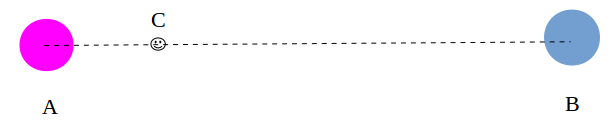
\includegraphics[width=0.6\textwidth]{nomor9.png}
\end{figure}

Andai diletakkan sebuah partikel uji di titik C bermassa $m$, maka berlaku:\\
\begin{eqnarray*}
\frac{GM_Bm}{(BC)^2}&=&\frac{GM_Am}{(AC)^2}\\
\frac{M_B}{(BC)^2}&=&\frac{M_A}{(10-BC)^2}\\
\left(\frac{10-BC}{BC}\right)^2&=&\frac{M_A}{M_B}\\
\frac{10}{BC}-1&=&\sqrt{\frac{M_A}{M_B}}\\
BC &=& \frac{10}{1 + \sqrt{\frac{M_A}{M_B}}}\\
BC &=& 7,5
\end{eqnarray*}
Jawaban seharusnya 7,5 au.




\question Hasil penelitian \textit{Supernova Cosmology Project} dan \textit{High-Z Supernova Search Team} adalah penemuan alam semesta mengembang dipercepat. Pengembangan alam semesta dipercepat diamati mulai dari \textit{redshift} $z\sim0,4$ setelah adanya peran \textit{dark energy}. Konsekuensi penemuan ini adalah
\begin{choices}
\choice kerapatan radiasi menurun sebanding dengan penurunan kerapatan \textit{dark energy}.
\choice kerapatan materi menurun sebanding dengan penurunan kerapatan \textit{dark energy}.
\choice kerapatan \textit{dark energy} menurun dengan cepat.
\choice kerapatan radiasi dan materi menurun dengan cepat.
\choice kerapatan \textit{dark energy} bertambah.
\end{choices}

\textit{Jawaban:} D

Berdasarkan model standar saat ini, komponen penyusun alam semesta terdiri dari radiasi, materi, dan \textit{dark energy}. Kerapatan radiasi dan materi sebagai pengisi alam semesta menurun cepat seiring mengembangnya alam semesta. Kerapatan \textit{dark energy}, khususnya jenis konstanta kosmologi, besarnya tetap selama pengembangan alam semesta. Hal ini yang menjelaskan percepatan pengembangan alam semesta.

\question Penentuan temperatur bintang yang benar adalah dengan cara
\begin{choices}
\choice mengukur terang semu bintang dan membuat diagram Hertzprung Russel untuk menentukan temperatur bintang
\choice mengukur indeks warna bintang dengan filter biru dan visual, dan menggunakan Hukum Wien untuk menentukan temperatur dari indeks warna
\choice untuk bintang yang dekat, mengukur paralaks dan menentukan jarak. Hubungkan jarak ini dengan temperatur.
\choice untuk beberapa bintang yang besar, mengukur diameternya dan menetapkan temperatur
\choice mengukur gerak bintang dalam sistem bintang ganda dan menggunakan Hukum Kepler untuk menentukan temperatur dari orbit bintang
\end{choices}

\textit{Jawaban:} B

Radiasi dari bintang dapat dianggap sebagai radiasi benda hitam. Temperatur bintang dapat diukur apabila kita mengetahui ``warna'' atau spektrumnya, sesuai dengan hukum Wien.



\question Pada saat hari proklamasi NKRI, fase Bulan ada di sekitar hari ke-8 atau ke-9. Diketahui bahwa 19 tahun surya bersesuaian dengan 235 periode sinodis Bulan (yang disebut siklus Meton). Tanggal 17 Agustus 2021 bertepatan dengan fase Bulan hari
\begin{choices}
\choice ke-8 atau ke-9
\choice ke-12 atau ke-13
\choice ke-2 atau ke-3
\choice ke-4 atau ke-5
\choice purnama
\end{choices}

\textit{Jawaban: A}\\
Proklamasi NKRI dilaksanakan pada tanggal 17 Agustus 1945. Tanggal 17 Agustus 2021 akan bertepatan dengan 4 kali kelipatan (bulat) siklus Meton.
$$\frac{2021-1945}{19} = 4$$
Setiap kelipatan siklus Meton ini, konfigurasi Bulan dan Bumi (terutama terkait fase Bulan) akan kembali seperti semula (``mirip''), sehingga pada tanggal 17 Agustus 2021, fase Bulan akan ada di hari ke-8 atau ke-9 juga.


\textit{Catatan}:\\
Jumlah hari dari 17 Agustus 1945 hingga 17 Agustus 2021.\\
Jumlah tahun kabisat: $\frac{2021-1945}{4}=19$\\
Jumlah hari dari tahun kabisat: $19\times 366=6954$ hari\\
Jumlah tahun basit: $2021-1945-\text{jumlah tahun kabisat}=57$\\
Jumlah hari dari tahun basit: $57\times 365=20805$ hari\\
Jumlah total hari: $6954+20805=27759$ hari\\

Jumlah hari dalam 1 siklus Meton: $235\times 29,5306=6939,691$ hari\\
Jumlah siklos Meton yang terlewati: $277759/6939,691=4,000034007\approx4$ kali.


\question Dua buah bintang, A dan B, dapat dianggap sebagai benda hitam sempurna. Jika kedua bintang mempunyai diameter yang sama, namun temperatur berbeda, masing-masing 8000 K dan 24000 K, maka perbandingan energi bintang A dan bintang B yang dipancarkan per satuan luas per satuan waktu adalah
\begin{choices}
\choice $\frac{1}{3}$
\choice $\frac{1}{9}$
\choice $\frac{1}{27}$
\choice $\frac{1}{81}$
\choice $\frac{1}{243}$
\end{choices}

\textit{Jawaban:} D\\
Energi yang dipancarkan benda hitam per satuan luas per satuan waktu dikenal sebagai besaran fluks pancaran yang sebanding dengan temperatur efektif bintang $T^4$ ($E = \sigma T^4$). Maka perbandingan besaran tersebut untuk bintang A terhadap bintang B: 
$$\left( \frac{T_A}{T_B}\right)^4=\left( \frac{8000}{24000}\right)^4=\frac{1}{81}$$ 




\question Which of the following stars is circumpolar in Romania (26\degree 0` E, 44\degree 25' N)
\begin{choices}
\choice $\zeta$ Herculis (16h 41m/+31\degree 36')
\choice $\beta$ Bootis (15h 01m/+40\degree 23')
\choice $\theta$ Aurigae (5h 59m/+37\degree 12')
\choice $\gamma$ Draconis (17h 56m/+51\degree 26')
\choice None of the stars above
\end{choices}

\textit{Jawaban: } D\\
For a star to be circumpolar from an observer on Earth, its declination ($\delta_*$) must satisfy: $\delta_*+\phi\geq $ 90\degree. With $\phi$ is the observer's latitude. Therefore, from Romania, circumpolar stars must have $\delta\geq $45\degree 35' and the correct answer is \textit{D}.




\vspace{0.5cm}
\textbf{Untuk satu soal berikut ini (No 15), jawablah}
\begin{choices}
\choice \textbf{jika 1, 2, dan 3 benar}
\choice \textbf{jika 1 dan 3 benar}
\choice \textbf{jika 2 dan 4 benar}
\choice \textbf{jika 4 saja benar}
\choice \textbf{jika semua benar}
\end{choices}

\question Sebuah objek ``aneh'' yang ditemukan oleh teleskop survey Pan-STARRS pada bulan Oktober 2017 diberi nama C/2017 U1 Oumuamua, menjadi pembicaraan ahli astronomi. Objek tersebut berada pada jarak 0,2 au dari Bumi saat pertama kali ditemukan dan bergerak menjauhi Matahari. Para astronom memperkirakan objek ini adalah sebuah komet yang berasal dari ruang antar bintang yang memasuki wilayah Tata Surya, akan tetapi dari ciri-ciri fisiknya lebih mendekati ciri-ciri sebuah asteroid. Beberapa karakteristik fisik objek Omuamua di bawah ini yang benar adalah
\begin{enumerate}
\item Objek ini memiliki orbit berbentuk parabola dan memiliki periode revolusi yang amat panjang sehingga dapat disimpulkan sebagai objek dari luar Tata Surya.
\item Objek ini memiliki orbit hiperbola yang memiliki eksentrisitas sebesar 1,2.
\item Oumuamua memiliki ciri sebuah komet tapi tidak memiliki ekor saat mendekati Matahari.
\item Oumuamua memiliki albedo yang kecil sehingga tidak dianggap sebagai komet.
\end{enumerate}

\textit{Jawaban: } C\\

Fakta-fakta mengenai C/2017 U1 Oumuamua dapat dibaca di \url{https://en.wikipedia.org/wiki/\%CA\%BBOumuamua}\\





\vspace{0.5cm}
\textbf{Soal Isian Singkat}

\question Apabila kita ingin meletakkan sebuah satelit ke orbit yang berada di atas permukaan Bulan, kecepatan terbang satelit tersebut adalah \ldots\ldots m/detik.

\textit{Jawaban:} $1679,66$

Kecepatan terbang satelit di atas permukaan Bulan: 
$$v=\sqrt{\frac{GM_{Bulan}}{R_{Bulan}}} = 1679,6556 \text{ m/detik}$$.



\question Kisi difraksi memiliki $10^4$ garis setiap 2,5 cm. Kisi difraksi ini disinari cahaya kuning dari lampu sodium ($\lambda_1=0,58959$ $\mu$m dan $\lambda_2=0,58900$ $\mu$m) pada arah normal. Sudut deviasi maksimum orde pertama untuk garis-garis sodium tersebut adalah \ldots\ldots derajat dan \ldots\ldots derajat.

\textit{Jawaban:} 13,641\degree dan 13,627\degree

Jarak antar garis pada kisi difraksi, 
$$d=\frac{2,5}{10^4} = 2,5\times 10^{-4} \text{  cm}$$

Persamaan umum untuk kisi difraksi, 
$$m\lambda=d(sin \theta_i+sin \theta_r)$$
dengan $m$ menyatakan orde, $\lambda$ panjang gelombang yang digunakan, $\theta_i$ sudut datang terhadap normal kisi, $\theta_r$ sudut pantul terhadap normal kisi.

Sudut datang pada arah normal mengindikasikan $\theta_i=0$\degree. Sehingga deviasi dapat langsung dinyatakan dengan sudut $\theta_r$.

\textit{Catatan}: samakan satuan $\lambda$ dan $d$ sebelum menghitung pada langkah selanjutnya.

Untuk orde pertama, $m=1$ atau $-1$, maka:
\begin{eqnarray*}
d \sin \theta_1 &=& m \lambda_1\\
2,5\times 10^{-4} \sin \theta_1 &=& 1 \cdot 0,58959\times 10^{-4}\\
\theta_1 &=& 13,641\\
d \sin \theta_2 &=& m \lambda_2\\
2,5\times 10^{-4} \sin \theta_2 &=& 1 \cdot 0,58900\times 10^{-4}\\
\theta_2 &=& 13,627
\end{eqnarray*}



\question Diketahui satelit Cassini memiliki massa 2,5 kg dan memiliki ukuran penampang 20 m$^2$. Pada tahun 2017, Cassini jatuh ke Saturnus. Asumsikan Cassini jatuh ke arah pusat Saturnus, kerapatan atmosfer Saturnus $9 \times 10^{-11}$ kg/m$^3$, dan koefisien gesek sebesar 2. Jika pada saat jatuh terjadi kesetimbangan antara gaya gravitasi dengan gaya gesek udara akibat ketebalan gas planet Saturnus, kecepatan jatuh Cassini pada saat kesetimbangan tersebut terjadi adalah \ldots\ldots\ldots km/detik.

Kecepatan ini disebut juga sebagai kecepatan terminal.


\textit{Jawaban: } 120,5

Gaya gesek dengan fluida biasa didefinisikan dengan persamaan,
\begin{equation*}
F_D = \frac{1}{2} \rho v^2 C_d A
\end{equation*}
dengan $\rho$ adalah rapat jenis fluida, $C_d$ adalah koefisien \textit{drag}/gesek, $A$ adalah luas penampang, dan $v$ adalah kecepatan benda.

Ketika kecepatan terminal tercapai (kecepatan jatuh menjadi konstan), terdapat kesetimbangan antara gaya gravitasi (berat Cassini di Saturnus) dan gaya gesek,
\begin{eqnarray*}
\frac{1}{2} \rho v^2 C_d A &=& \frac{GM_\text{Saturn} m_\text{Cassini}}{r^2}\\
v_\text{terminal} &=&  \sqrt{\frac{2 GM_\text{Saturn} m_\text{Cassini}}{\rho C_d A r^2}}\\
v_\text{terminal} &=& 120493,5 \text{ m/s} = 120,5 \text{ km/s}
\end{eqnarray*}

\textit{Catatan}: diasumsikan bahwa kecepatan terminal terjadi tidak jauh dari permukaan Saturnus, $r =$ radius planet Saturnus.





\question Jika mata manusia memiliki diameter pupil 4,5 mm, maka sebuah refraktor dengan diameter lensa objektif 45 cm memberikan daya pisah dan daya kumpul cahaya dalam panjang gelombang visual (550 nm), masing-masing sebesar \ldots\ldots  kali dan \ldots\ldots kali lebih baik daripada mata.

\textit{Jawaban: } 100 dan 10000
\begin{itemize}
\item Daya pisah ditentukan dengan
$$\theta_{\text{res}} = \frac{1,22 \lambda}{D}$$
berbanding terbalik dengan diameter.

\begin{eqnarray*}
\frac{\theta_\text{teleskop}}{\theta_\text{mata}} &=& \frac{D_\text{mata}}{D_\text{teleskop}} = \frac{4,5}{450} = 0,01
\end{eqnarray*}

\textit{Hati-hati}: semakin kecil $\theta_{\text{res}}$, maka daya pisahnya semakin ``baik''!

Teleskop ini memiliki daya pisah 100 kali lebih baik daripada mata.


\item Kemampuan mengumpulkan cahaya (\textit{light gathering power}, LGP) sebanding dengan luas penampang (area) pengumpul, atau
$$LGP \propto D^2$$

$$\frac{LGP_\text{teleskop}}{LGP_\text{mata}} = \left( \frac{450}{4,5} \right)^2 = 10000$$

Teleskop ini memiliki daya kumpul cahaya 10000 kali lebih baik daripada mata.

\end{itemize}




\question Citra Matahari yang disertai bintik Matahari diperoleh dari pengamatan resolusi tinggi dalam cahaya tampak. Fotometri dari bintik Matahari ini menunjukkan bahwa kecerlangan permukaan bintik Matahari adalah sekitar 0,32 kali kecerlangan permukaan fotosfer sekitarnya. Jika temperatur fotosfer Matahari diketahui sekitar 6600 K, temperatur bintik Matahari adalah \ldots\ldots K.

\textit{Jawaban: } 4964

Asumsikan bintik Matahari dan fotosfer sebagai benda hitam sempurna,
\begin{eqnarray*}
\frac{E_\text{sunspot}}{E_\text{fotosfer}} &=& \frac{\sigma T^4_\text{sunspot}}{\sigma T^4_\text{fotosfer}}\\ 
0,32 &=& \left( \frac{T_\text{sunspot}}{T_\text{fotosfer}} \right)^{4}\\
\frac{T_\text{sunspot}}{T_\text{fotosfer}} &=& 0,7521\\
T_\text{sunspot} &=& 4964 \text{ K}
\end{eqnarray*}


\end{questions}


\vspace{2cm}
\begin{flushright}
Solusi seperti ini dapat diperoleh di \url{http://ridlow.wordpress.com}
\end{flushright}
\end{document}
